\documentclass{standalone}
\usepackage{tikz}
\usepackage{circuitikz}\usetikzlibrary{arrows,calc,decorations.markings,decorations.pathreplacing,positioning}
\begin{document}
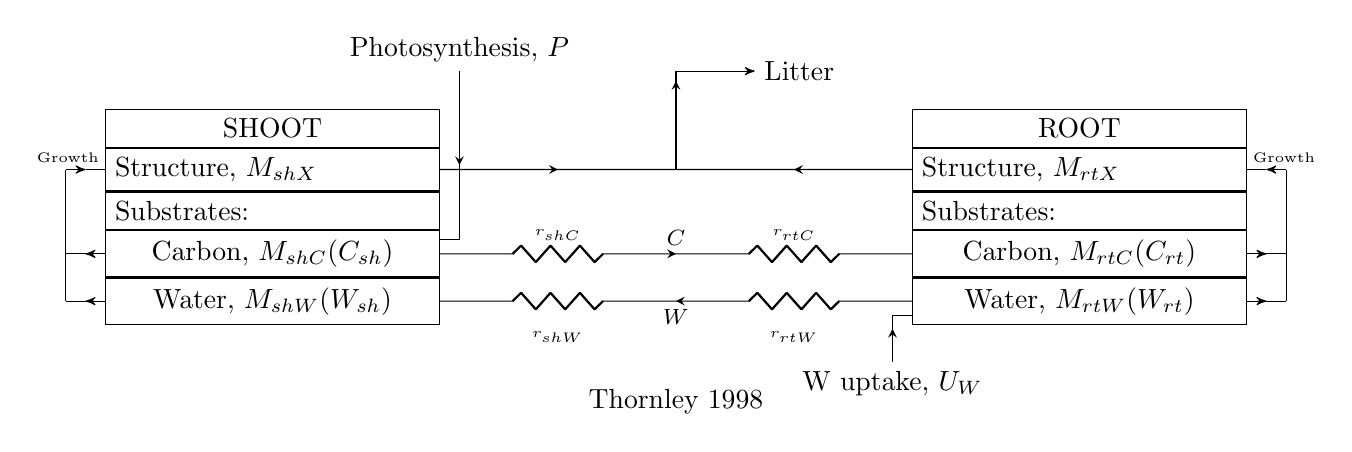
\begin{tikzpicture}[>=stealth', transform shape]
\newcommand{\pbox}[1][]{\node [#1, draw, text width=4cm]}
\coordinate (c);
\pbox [left=3cm of c, align=center] (S) {SHOOT};
\pbox [below=0cm of S] (S0) {Structure, $M_{shX}$};
\pbox [below=0cm of S0] (S1) {Substrates:};
\pbox [below=0cm of S1, align=center] (S2) {Carbon, $M_{shC} (C_{sh})$};
\pbox [below=0cm of S2, align=center] (S3) {Water, $M_{shW} (W_{sh})$};

\pbox [right=3cm of c, align=center] (R) {ROOT};
\pbox [below=0cm of R] (R0) {Structure, $M_{rtX}$};
\pbox [below=0cm of R0] (R1) {Substrates:};
\pbox [below=0cm of R1, align=center] (R2) {Carbon, $M_{rtC} (C_{rt})$};
\pbox [below=0cm of R2, align=center] (R3) {Water, $M_{rtW} (W_{rt})$};



\def\dx{.25}
\newcommand{\growth}[3]{
  \def\sgn{#3}
  \draw [->] (#12.#2) -- ++(\sgn*\dx,0);
  \draw [->] (#13.#2) -- ++(\sgn*\dx,0);
  \draw [<-] (#10.#2) ++(\sgn*\dx,0) -- node [yshift=.15cm, xshift=\sgn*.1cm] {\tiny Growth} ++(\sgn*\dx,0);
  \draw (#12.#2) ++(\sgn*\dx,0) -- ++(\sgn*\dx,0);
  \draw (#13.#2) ++(\sgn*\dx,0) -- ++(\sgn*\dx,0);
  \draw (#10.#2) -- ++(\sgn*\dx,0);
  \draw (#10.#2) -- ++(\sgn*\dx,0);
  \draw (#12.#2) ++(\sgn*2*\dx, 0) -- ($(#10.#2)+(\sgn*2*\dx,0)$);
  \draw ($(#13.#2)+(\sgn*2*\dx,0)$) -- ($(#12.#2)+(\sgn*2*\dx,0)$);
}
\growth{S}{west}{-1};
\growth{R}{east}{1};

\begin{scope} 
\tikzset{
  mid arrow/.style={postaction={decorate,decoration={
        markings,
        mark=at position .5 with {\arrow[#1]{stealth}}
      }}},
}
\ctikzset{bipoles/resistor/height=0.15}
\draw [mid arrow]
  (S2) -- ($(S2.east)!.15!(R2.west)$) to [R=\tiny$r_{shC}$] ($(S2.east)!.35!(R2.west)$)
       -- ($(S2.east)!.5!(R2.west)$) node [yshift=.2cm] {\footnotesize $C$}
       -- ($(S2.east)!.65!(R2.west)$) to [R=\tiny$r_{rtC}$] ($(S2.east)!.85!(R2.west)$)
       -- (R2);
           
\draw [mid arrow]
  (R3) -- ($(S3.east)!.85!(R3.west)$) to [R=\tiny$r_{rtW}$] ($(S3.east)!.65!(R3.west)$)
       -- ($(S3.east)!.5!(R3.west)$) node [yshift=-.2cm] {\footnotesize $W$}
       -- ($(S3.east)!.35!(R3.west)$) to [R=\tiny$r_{shW}$] ($(S3.east)!.15!(R3.west)$)
       -- (S3);
           
\node (Uw) at ($(R3.south west)-(\dx,3*\dx)$) {W uptake, $U_W$};
\draw [mid arrow] (Uw) |- (R3.185);

\node (Uc) at ($(S0.north east)+(\dx, 5*\dx)$) {Photosynthesis, $P$};
\draw [mid arrow] (Uc) |- (S2.5);

\draw [mid arrow] (S0) -- ($(S0)!.5!(R0)$);
\draw [mid arrow] (R0) -- ($(S0)!.5!(R0)$);
\draw [mid arrow,->] ($(S0)!.5!(R0)$) -- ++(0,5*\dx) -- ++(1, 0) node [anchor=west] {Litter};

\coordinate (l) at ($(S3)!.5!(R3)$);
\node [below=1cm of l] {Thornley 1998};
\end{scope}
           
\end{tikzpicture}
\end{document}
